\documentclass[10pt]{beamer}
%\documentclass[10pt,handout]{beamer} % This is to create a printout!!!!!

\mode<presentation>

\usetheme{Madrid}
%\definecolor{lightblue}{HTML}{3498DB}
\definecolor{lightblue}{HTML}{5DADE2}
%\definecolor{colblue2}{HTML}{0072CE} % Juan's blue
\usecolortheme[named=lightblue]{structure}
\setbeamercolor{button}{fg=white, bg=lightblue}

%\usecolortheme{seahorse}
%\usecolortheme{rose}
\usefonttheme[onlylarge]{structuresmallcapsserif}
%\usefonttheme[onlymath]{serif}

\definecolor{alertcolor}{rgb}{0.8,0,0} % dark red
%\definecolor{alertcolor}{HTML}{5DADE2} % light blue
\newcommand{\hl}[1]{\textcolor{darkred}{#1}}
\definecolor{beamer@darkred}{rgb}{0.8,0,0}
\setbeamercolor{alerted text}{fg=beamer@darkred}

\renewcommand{\baselinestretch}{1.3}   
\setbeamersize{text margin left=0.5cm}
\setbeamersize{text margin right=0.5cm}

\setbeamertemplate{itemize items}[boadilla]
\setbeamertemplate{enumerate items}[default]
%\usepackage[english]{babel}
%\usepackage[latin1]{inputenc}
\usepackage{times}
\usepackage[T1]{fontenc}
\usepackage{graphicx}
\usepackage{appendixnumberbeamer}
\usepackage{epstopdf}
%\usepackage{econometrics}
\usepackage{tikz}
\usetikzlibrary{calc}
\usepackage{booktabs}
\usepackage{tabularx}
\usepackage{subcaption}
\usepackage[makeroom,thicklines]{cancel}

\usepackage{multirow}
\usepackage{rotating}
\usepackage{array}
\usepackage{float}

%\setbeamercovered{transparent}
\setbeamercovered{invisible}
\usenavigationsymbolstemplate{}
\usepackage{appendixnumberbeamer}

\setbeamertemplate{itemize items}[boadilla]
\setbeamertemplate{enumerate items}[default]

\newcolumntype{P}[1]{>{\centering\arraybackslash}p{#1}}


\title[Phillips Curve]{Phillips Curve: Cross-Sectional Estimation}
\author[Nakamura, Steinsson]{Emi Nakamura and J\'{o}n Steinsson\thanks{These slides build heavily on slides for our paper Hazell, Herreno, Nakamura, Steinsson (2021)}}
\institute[Berkeley]{UC Berkeley}
\date{October 2021}

\begin{document}


\begin{frame}
  \titlepage
\end{frame}


\begin{frame}{Phillips Curve}
	New Keynesian formalization:
	\[ \pi_{t} = \beta E_{t} \pi_{t+1} - \kappa (u_{t} - u_{t}^{n} ) + \nu_{t} \]
	Drivers of inflation:
	\begin{itemize}
		\item Expected inflation: $E_{t} \pi_{t+1}$
		\item Measure of ``output gap'': $u_{t} - u_{t}^{n}$
		\item Cost-push shocks: $\nu_t$
	\end{itemize}
	\vspace{10pt}
	\vspace{10pt}
	Object of interest: Slope coefficient $\kappa$
	\begin{itemize}
		\item How much does an increase in ``demand'' affect inflation 
	\end{itemize}
\end{frame}


\begin{frame}{Conventional Wisdom}
	\begin{itemize}
		\itemsep1em 
		\item Volcker disinflation:
		\begin{itemize}
			\item Tight policy -> high unemployment -> lower inflation
			\item Substantial slope of the Phillips curve
		\end{itemize} 
		\item Since 1990:
		\begin{itemize}
			\item Muted response of inflation to unemployment
			\item Great Recession: missing disinflation 
			\item Late 2010s and 1990s: missing rise in inflation
		\end{itemize}
		\item Phillips curve is getting flatter or hibernating
		\begin{itemize}
			\item Perhaps an important flaw in the Keynesian model
		\end{itemize}
	\end{itemize}
\end{frame}


\begin{frame}{Conventional Wisdom}
	\begin{itemize}
		\itemsep1em 
		\item Assume adaptive expectations: $\beta E_{t} \pi_{t+1} = \pi_{t-1}$
		\item In this case, 
		\[ \pi_{t} = \beta E_{t} \pi_{t+1} - \kappa (u_{t} - u_{t}^{n} ) + \nu_{t} \]
		becomes
		\[ \Delta \pi_{t} = - \kappa (u_{t} - u_{t}^{n} ) + \nu_{t}, \]		 
		\item Stock and Watson (2019):
		\begin{itemize}
			\item $\Delta \pi_{t}$: Annual change in 12-month core PCE inflation 
			\item $u_{t} - u_{t}^{n}$: CBO unemployment gap  
			\item Refer to $\kappa$ as ``Phillips correlation''
		\end{itemize}
	\end{itemize}
\end{frame}


\begin{frame}{Flattening Phillips Curve}
	\begin{figure}
		\centering
		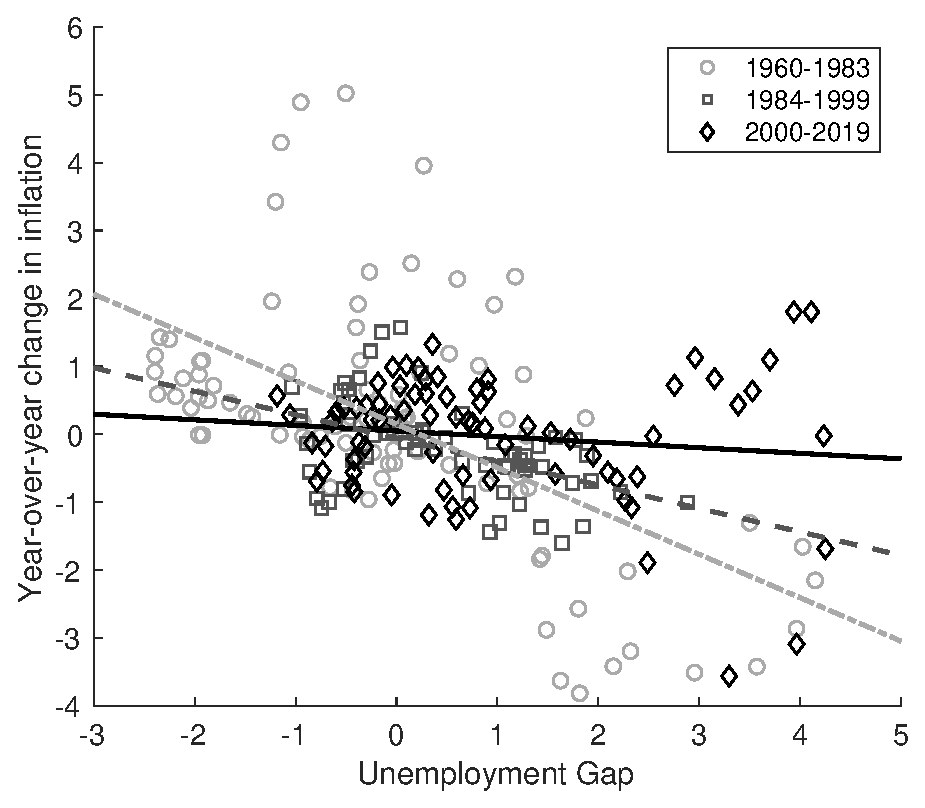
\includegraphics[height = 0.84 \textheight]{FiguresTables/Fig_stock_watson.eps}
	\end{figure}
	%Data are quarterly. The year-over-year change in inflation plotted on the vertical axis is the four-quarter change of the (backwards-looking) four-quarter moving average of the inflation rate. The horizontal axis plots the (backwards-looking) four-quarter moving average of the CBO unemployment gap.
\end{frame}


\begin{frame}{Alternative Explanation}
	\begin{itemize}
		\itemsep1em 
		\item Volcker disinflation:
		\begin{itemize}
			\item Sharp regime shift
			\item Rapid fall in long-run inflation expectations
			\item Rapid fall in inflation
		\end{itemize}
		\item Since 1990:
		\begin{itemize}
			\item Long-run inflation expectations have become anchored
			\item Consequently, inflation has become more stable
		\end{itemize}
		\item Apparent ``flattening'' of Phillips curve due to anchoring of \\ inflationary expectations {\small (Bernanke, 2007; Mishkin, 2007)}
	\end{itemize}
\end{frame}


\begin{frame}{Long-Run Inflation Expectations}
	\begin{figure}
		\centering
		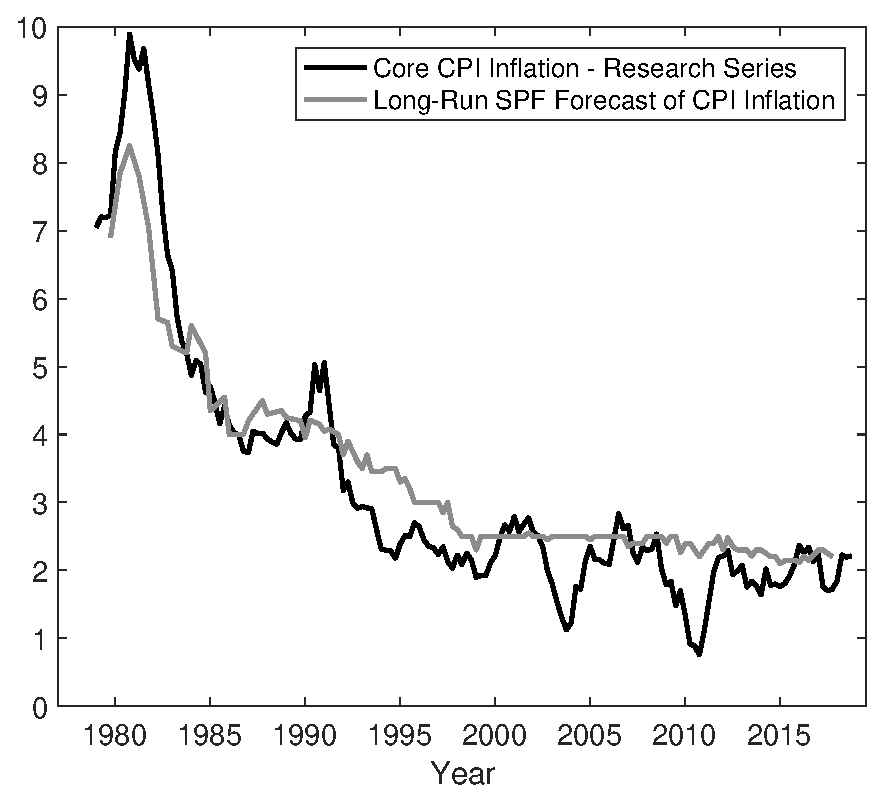
\includegraphics[height = 0.84 \textheight]{FiguresTables/Fig_plot_inf_expinf_lt.eps}
	\end{figure}
\end{frame}


\begin{frame}{Can We Tell These Stories Apart?}
	\begin{itemize}
		\itemsep1em 
		\item Extremely difficult using aggregate evidence
		\begin{itemize}
			\item Results based on survey or adaptive expectations are very sensitive to details of specification (e.g., which expectation variable)
			\item Results based on structural rational expectations specifications also very sensitive to details (partly due to a weak instruments problem) 
		\end{itemize}
		\item Mavroeidis, Plagborg-Moller, Stock 14:
		
		\vspace{5pt}
		\begin{quote}
			{\small [T]he Literature has reached a limit on how much can be learned about the New Keynesian Phillips curve from aggregate macroeconomic time series. New identification approaches and new datasets are needed to reach an empirical consensus.}
		\end{quote}
	\end{itemize}
\end{frame}


\begin{frame}{Identification Challenges}
	\begin{enumerate}
		\itemsep1em 
		\item Inflation expectations may covary with unemployment
		\begin{itemize}
			\item For example: Imperfectly credible regime change
			\item Literature seeks to control for inflation expectations \\ but this is difficult in practice 
		\end{itemize}
		\item Supply shocks ($u^n_t$ and $\nu_t$)
		\begin{itemize}
			\item Lead to positive comovement between inflation and unemployment (stagflation)
			\item Good monetary policy compounds with by counteracting demand variation, leaving only supply variation \\ (Fitzgerald-Nicolini, 2014, McLeay-Tenreyro 2019)
		\end{itemize}
	\end{enumerate}
\end{frame}


\begin{frame}{Can Cross-Sectional Data Help?}
	\begin{itemize}
		\itemsep1em
		\item Recent literature estimates ``regional Phillips curves''
		\begin{itemize}
			\item Fitzgerald-Nicolini 14; Kiley 15; Babb-Detmeister 17; McLeay-Tenreyro 19; Hooper-Mishkin-Sufi 19; Fitzgerald-Jones-Kulish-Nicolini 20; Beraja-Hurst-Ospina 19 (wages), Hazell-Herreno-Nakamura-Steinsson 21.
		\end{itemize}
		\item Major advantages:
		\begin{itemize}
			\item Fixed effects soak up variation in (common) long-run inflation expectations
			\item Fixed effects soak up aggregate supply shocks
			\item Shift-share instruments can be used to deal with regional supply shocks
		\end{itemize}
		\item New challenge:
		\begin{itemize}
			\item How is the slope of the regional Phillips curve related to the slope of the aggregate Phillips curve? 
		\end{itemize}
	\end{itemize}
\end{frame}

\begin{frame}{The Role of the Long-Run Inflation Target}
	\begin{itemize}
		\itemsep1em 
		\item Let's understand better the central role of long-run inflation expectations:
		\[\pi_{t}=\beta E_{t}\pi_{t+1}-\kappa (u_{t} - u_t^n)  + \nu_{t}  \]
		\item Solve forward:
		\[\pi_{t}=-\kappa E_{t}\sum_{j=0}^{\infty}\beta^{j} u_{t+j} + \omega_{t}\]
		where $\omega_t = E_t\sum_{j=0}^{\infty}\beta^{j}(\kappa u_{t+j}^{n} + \nu_{t+j})$. 
		\item Looks like long-run inflation expectation vanishes due to discounting
		\item This is an illusion!
	\end{itemize}
\end{frame}	 


\begin{frame}{The Role of the Long-Run Inflation Target}
	\begin{itemize}
		\item Useful to decompose $u_{t+j}$ into permanent and transitory component:
		\[\pi_{t}=-\kappa E_{t}\sum_{j=0}^{\infty}\beta^{j} u_{t+j} + \omega_{t}\]
		becomes
		\[\pi_{t}=-\kappa E_{t}\sum_{j=0}^{\infty}\beta^{j}\tilde{u}_{t+j} + \frac{\kappa}{1-\beta}E_{t} u_{t+\infty} + \omega_{t}\]
		where $\tilde{u}_{t}\equiv u_{t}- E_{t}u_{t+\infty}$
		\item Since $\frac{\kappa}{1-\beta} E_{t}u_{t+\infty}=E_{t}\pi_{t+\infty}$, we have
		\[\pi_{t}=-\kappa E_{t}\sum_{j=0}^{\infty}\beta^{j}\tilde{u}_{t+j} + E_{t}\pi_{t+\infty} + \omega_{t}\]
		(Same result with $\beta = 1$)
	\end{itemize}
\end{frame}


\begin{frame}{The Role of the Long-Run Inflation Target}
	\[\pi_{t}=-\kappa E_{t}\sum_{j=0}^{\infty}\beta^{j}\tilde{u}_{t+j} + E_{t}\pi_{t+\infty} + \omega_{t}\]
		\begin{itemize}
		\itemsep1em 
		\item Long-run inflation target actually major determinant of current inflation
		\item Has a coefficient of one!!
		\item Current inflation moves one-for-one with beliefs about \\ long-run inflation target
		\item In contrast, $\kappa$ may be very small
	\end{itemize}
\end{frame}


\begin{frame}{The Role of the Long-Run Inflation Target}
	\begin{itemize}
		\itemsep1em 
		\item To simplify, one can assume that $\tilde{u}_t$ follows an AR(1)
		\item This implies $E_t \tilde{u}_{t+j} = \rho^j_u \tilde{u}_{t}$
		\[\pi_{t}=-\kappa E_{t}\sum_{j=0}^{\infty}\beta^{j}\tilde{u}_{t+j} + E_{t}\pi_{t+\infty} + \omega_{t}\]
		becomes
		\[ \pi_{t} = - \psi \tilde{u}_{t} + E_{t}\pi_{t+\infty} + \omega_t\]
		where $\psi = \kappa / (1-\beta\rho_{u})$. 
	\end{itemize}
\end{frame}


\begin{frame}{The Role of the Long-Run Inflation Target}
	\[ \pi_{t} = - \psi \tilde{u}_{t} + E_{t}\pi_{t+\infty} + \omega_t\] \vspace{-10pt}	
	\begin{itemize}
		\itemsep1em
		\item Variation in inflation may be dominated by variation in $E_t \pi_{t+\infty}$
		\item Variation in inflation may be \textbf{completely unrelated} to variation in $\tilde{u}_{t}$
		\item Worse still, correlation between $E_{t}\pi_{t+\infty}$ and $\tilde{u}_t$ potentially a source of \\ severe omitted variables bias
	\end{itemize}
\end{frame}	  
	  


\begin{frame}{How Different Are $\pi_t$ and $E_t \pi_{t+1}$?}
\[ \pi_{t} = \beta E_{t} \pi_{t+1} - \kappa (u_{t} - u_{t}^{n} ) + \nu_{t} \]
\vspace{-10pt}
\begin{itemize}
	\itemsep1em
	\item This is approximately (if $\beta \approx 1$): 
	\[ \pi_{t} - E_{t} \pi_{t+1} \approx - \kappa (u_{t} - u_{t}^{n} ) + \nu_{t} \] 
	\item So, standard analysis aims to explain $\pi_{t} - E_{t} \pi_{t+1}$
	\item But how much is there to explain?
	\item Let's look at the difference between $\pi_t$ and $E_t \pi_{t+1}$ in the data 
\end{itemize}
\end{frame}


\begin{frame}
	\begin{figure}
		\centering
		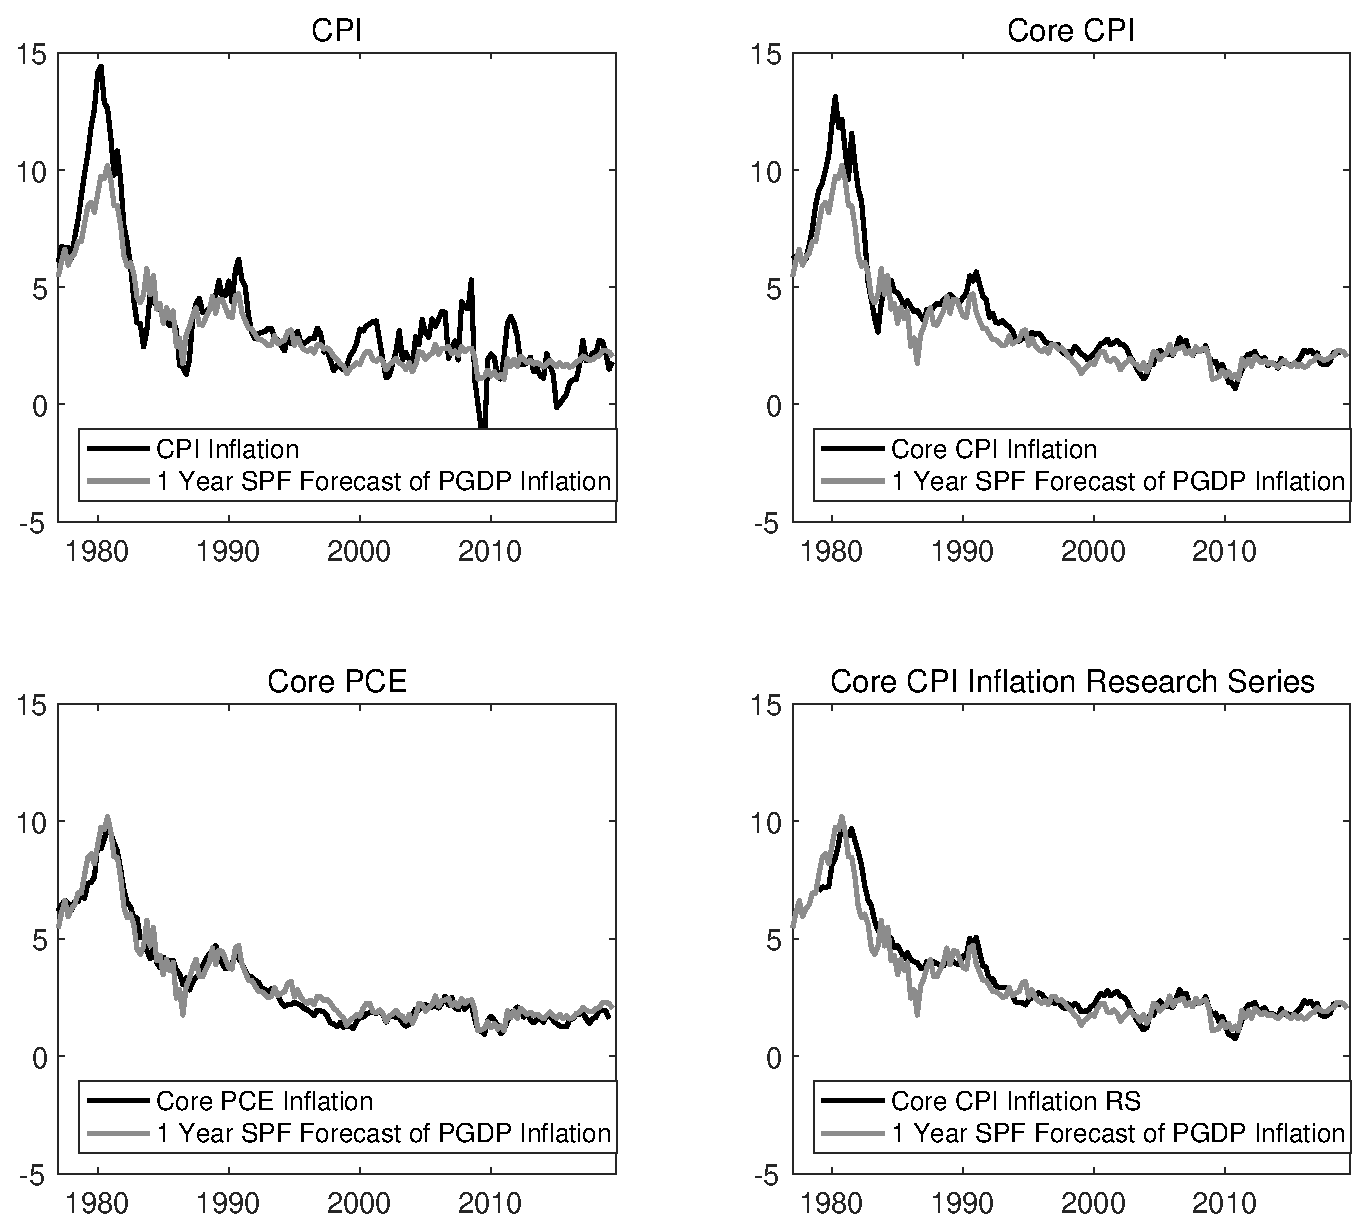
\includegraphics[width=0.84\textwidth]{FiguresTables/Fig_subplots_inf_expinf.eps}
	\end{figure}
\end{frame}


\begin{frame}{ $\pi_{t} \approx E_{t} \pi_{t+1}$}
\[ \pi_{t} - E_{t} \pi_{t+1} \approx - \kappa (u_{t} - u_{t}^{n} ) + \nu_{t} \]
	\begin{itemize}
		\item Inflation gap for core inflation is small throughout \\ {\small (for core using modern methods)}
		\item Consistent with a flat Phillips curve
	\end{itemize}

\vspace{10pt}
However:
	\begin{itemize}
		\item Relies heavily on exact timing of New Keynesian Phillips curve \\ {\small (Also subject to other concerns regarding aggregate Phillips curve estimation)}
	\end{itemize}
\end{frame}


\begin{frame}{A Model of the Regional Phillips Curve}
	\begin{itemize}
		\itemsep1em 
		\item Two regions: Home and Foreign
		\item Tradeable and non-tradeable sector in each region
		\item No labor mobility between regions
		\item Perfect labor mobility between sectors within region
		\item Monetary union
	\end{itemize}
\end{frame}


\begin{frame}{Households and Firms}
	\begin{itemize}
		\itemsep1em
		\item Households:
		\begin{itemize}
			\item Consume and supply labor
			\item Nested CES demand over varieties of traded and non-traded goods
			\item GHH preferences 
		\end{itemize}
		\item Firms:
		\begin{itemize}
			\item Linear production function in labor 
			\item Calvo (1983) type price rigidity
		\end{itemize}
	\end{itemize}
\end{frame}


\begin{frame}{Phillips Curves}
	\begin{itemize}
		\itemsep1em 
		\item Regional Phillips Curve for Non-Tradeables:
		\[\pi^N_{Ht}=\beta E_{t}\pi^N_{H,t+1}-\kappa\hat{u}_{Ht} - \lambda \hat{p}^N_{Ht} + \nu^N_{Ht} \]
		\item Aggregate Phillips Curve:
		\[\pi_{t}=\beta E_{t} \pi_{t+1} - \kappa\hat{u}_{t} + {\nu}_{t} \]
		where $\hat{u}_{Ht} = - \hat{n}_{Ht}$ and $\hat{u}_t = - \hat{n}_t$ 
		\item Important result: Same slope $\kappa$
		\begin{itemize}
			\item This is true for non-tradeable regional Phillips curve
			\item Not for overall regional Phillips curve (traded goods priced nationally)
			\item Relies on GHH preferences
		\end{itemize}	
	\end{itemize}		
\end{frame}


\begin{frame}{Regional Phillips Curve for Non-Tradeables}
	\[\pi^N_{Ht}=\beta E_{t}\pi^N_{H,t+1}-\kappa\hat{u}_{Ht} - \lambda \hat{p}^N_{Ht} + \nu^N_{Ht} \]
	\vspace{-10pt}
	\begin{itemize}
		\itemsep1em 
		\item Extra term: $\lambda \hat{p}^N_{Ht}$. Theoretically important!
		\item Common critique:
		\begin{itemize}
			\item Even in multi-region RBC model, regional demand shock would result in an increase in relative price of local goods
		\end{itemize}
		\item Extra term implies that this model nests multi-region RBC model
		\item If prices were flexible, $\lambda$ would be large
		\item Empirically, $\lambda$ estimated to be small
	\end{itemize}
\end{frame}


\begin{frame}{Regional Phillips Curve Solved Forward}
	\begin{itemize}
		\itemsep1.5em 
		\item Let's solve the regional Phillips curve forward:
		\[\pi_{Ht}^N = - \kappa E_{t} \sum_{j=0}^{\infty} \beta^j  \tilde{u}_{H,t+j} - \lambda E_{t} \sum_{j=0}^{\infty} \beta^j \hat{p}_{H,t+j}^N + E_{t}\pi_{t+\infty} + \omega_{Ht}^N, \]
		\item Long-run inflation expectations are constant across regions \\ and can be replaced with time and state fixed effects:
		\[\pi_{Ht}^N = - \kappa E_{t} \sum_{j=0}^{\infty} \beta^j  \tilde{u}_{H,t+j} - \lambda E_{t} \sum_{j=0}^{\infty} \beta^j \hat{p}_{H,t+j}^N + \alpha_i + \gamma_t + \omega_{Ht}^N, \]
		\item Panel specification ``differences out'' long-run inflation expectations
	\end{itemize}
\end{frame}


\begin{frame}{Common Across Regions?}
	\[\pi_{Ht}^N = - \kappa E_{t} \sum_{j=0}^{\infty} \beta^j  \tilde{u}_{H,t+j} - \lambda E_{t} \sum_{j=0}^{\infty} \beta^j \hat{p}_{H,t+j}^N + E_{t}\pi_{t+\infty} + \omega_{Ht}^N, \]
	\vspace{-10pt}
	\begin{itemize}
		\itemsep1em 
		\item Can't long-run inflation expectation differ across regions?
		\begin{itemize}
			\item Prices are rising in New York relative to Kansas
			\item Balassa-Samuelson effects 
		\end{itemize}
		\item Constant differences captured by state fixed effects
		\item Non-constant differences in \textbf{long-run} inflation expectations \\ will be in error term
		\begin{itemize}
			\item Small part of total variation (arguably)
			\item A concern if correlated with instruments
		\end{itemize}
	\end{itemize}
\end{frame}


\begin{frame}{Interpretation of Slope Coefficient}
	\begin{itemize}
		\itemsep1em 
		\item Regional Phillips curve:
		\[\pi_{Ht}^N = - \textcolor{purple}{\boldsymbol{\kappa}} E_{t} \sum_{j=0}^{\infty} \beta^j  \tilde{u}_{H,t+j} - \lambda E_{t} \sum_{j=0}^{\infty} \beta^j \hat{p}_{H,t+j}^N + \alpha_i + \gamma_t + \omega_{Ht}^N, \]
		\item Suppose we assume that $\tilde{u}_{Ht}$ and $\hat{p}_{Ht}^N$ follow AR(1) processes:
		\begin{equation} \label{emp spec} 
			\pi_{Ht}^N = - \textcolor{purple}{\boldsymbol{\psi}} \tilde{u}_{Ht} - \delta \hat{p}_{Ht}^N + \alpha_i + \gamma_t + \omega_{Ht}^N
		\end{equation} 
		\[ \text{where} \;\;\;\;\;\; \psi = \frac{\kappa}{1-\beta\rho_{u}} \;\;\;\;\;\; \text{and} \;\;\;\;\;\; \delta = \frac{\lambda}{1-\beta\rho_{pN}} \]
		\item Equation \eqref{emp spec} similar to typical regional empirical specification
		\item But $\kappa$ and $\psi$ are not the same! 
		\begin{itemize}
			\item $\psi$ potentially much larger than $\kappa$ since $\tilde{u}_{Ht}$ is persistent
			\item Prior regional Phillips curve literature estimates $\psi$ not $\kappa$.
			\item Helps explain large slope estimates in this literature  
		\end{itemize}
	\end{itemize}
\end{frame}


\begin{frame}{Data}
	\begin{itemize}
		\itemsep1em
		\item New state-level inflation indexes {\small (Hazell-Herreno-Nakamura-Steinsson 21)}
		\begin{itemize}
			\item Sample period 1978 - 2018, quarterly
			\item Based on BLS CPI micro data 
			\item Free of cross-state imputations
			\item Separate indexes for tradeables vs. non-tradeables
		\end{itemize}
		\item Analyze housing separately
		\item Measure of slack: State unemployment rates
		\item Tradeable demand spillover instrument:
		\begin{itemize}
			\item State-industry employment shares
			\item 2-digit SIC for 1975-2000
			\item 3-digit NAICS from 1990-2018
		\end{itemize}
	\end{itemize}
\end{frame}


\begin{frame}[label=regbc]{Regional Business Cycles}
	\begin{figure}
		\centering 
		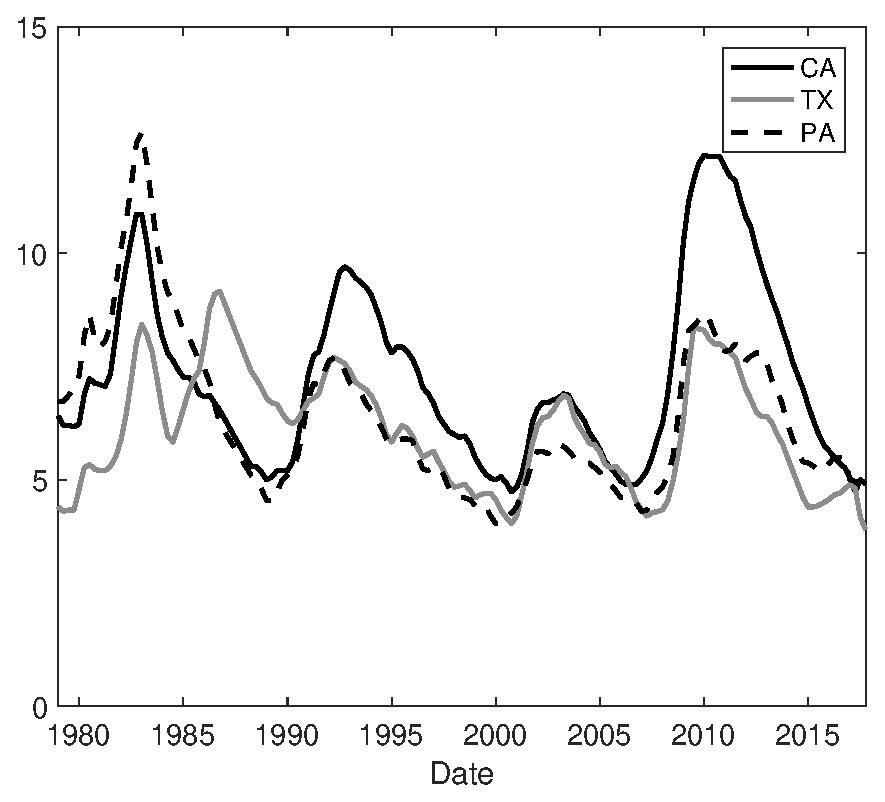
\includegraphics[width = 0.7\textwidth]{FiguresTables/Fig_une_cs}
	\end{figure}
\end{frame}


\begin{frame}{Phillips Curve Slope}
	\begin{itemize}
		\item Regional Phillips curve from model:
		\[\pi_{it}^N = \alpha_i + \gamma _t - \textcolor{purple}{\boldsymbol{\kappa}} E_t \sum_{j=0}^{\infty} \beta^j u_{i,t+j} - \lambda E_t \sum_{j=0}^{\infty} \beta^j \hat{p}^N_{i,t+j} + \omega_{it} \]
		\item Reduced form equation similar to prior literature:
		\[ \pi_{it}^{N} = \alpha_i + \gamma_{t} - \textcolor{purple}{\boldsymbol{\psi}} u_{i,t-4} - \delta p_{i,t-4}^{N} + \varepsilon_{it} \] \vspace{-15pt}
		\item HHNS present estimates of both $\textcolor{purple}{\boldsymbol{\kappa}}$ and $\textcolor{purple}{\boldsymbol{\psi}}$
	\end{itemize}
\end{frame}


\begin{frame}{Estimation of $\kappa$}
	\[\pi_{it}^N = \alpha_i + \gamma _t - \textcolor{purple}{\boldsymbol{\kappa}} E_t \sum_{j=0}^{\infty} \beta^j u_{i,t+j} - \lambda E_t \sum_{j=0}^{\infty} \beta^j \hat{p}^N_{i,t+j} + \omega_{it} \] \vspace{-10pt}
	\begin{itemize}
		\itemsep1em 
		\item Replace expectations with realized values and expectation error \\ and truncate the infinite sums:
		\[\pi_{it}^N = \alpha_i + \gamma _t - \textcolor{purple}{\boldsymbol{\kappa}} \sum_{j=0}^{T} \beta^j u_{i,t+j} - \lambda \sum_{j=0}^{T} \beta^j \hat{p}^N_{i,t+j} + \omega_{it} + \eta_{it} \]
		where $\eta_{it}$ is an expectations error (and truncation error)
		\item $\kappa$ can now be estimated using an IV regression (i.e., GMM) \vspace{5pt}
		\item Calibrate $\beta = 0.99$
	\end{itemize}
\end{frame}


\begin{frame}{Identification} \label{identification}
	Two Approaches: \vspace{10pt}
	\begin{enumerate}
		\itemsep1em 
		\item Use lagged unemployment and relative prices as instruments
		\begin{itemize}
			\item Unemployment may reflect supply shocks
			\item Time fixed effects capture national supply shocks
			\item Identifying assumption: No relative change in restaurant technology in Texas vs. Illinois when Texas experiences a recession relative to Illinois
		\end{itemize}
		\item Tradeable demand instrument
	\end{enumerate}
\end{frame}


\begin{frame}{Tradeable Demand Spillover Instrument} \label{IV}
	\[\text{Tradable Demand}_{i,t} = \sum_{x \in T} \bar{S}_{x,i} \times \Delta \log{S}_{-i,x,t}\] \vspace{-12pt} 
	
	\begin{itemize}
		\itemsep0.5em
		\item $\bar{S}_{x,i}$: Average employment share of industry $x$ in state $i$ over time \vspace{-0.5em}			
		\item $\log S_{-i,x,t}$: National employment share of industry $x$ at time $t$
	\end{itemize}	
	
	\begin{itemize}
		\item Identifying assumption: supply shocks not simultaneously correlated with \textbf{both} shifts $ \Delta \log S_{-i,x,t}$ \textbf{and} shares $\bar{S}_{x,i}$ 
		\item Intuition:
		\begin{itemize}
			\item Oil boom increases labor demand and wages in Texas
			\item ``Demand shock'' for Texan restaurants
			\item Oil boom does not differentially affect production technology for restaurants in Texas
		\end{itemize}		
	\end{itemize}			
\end{frame}


\begin{frame}{Estimation of $\psi$}
	\[ \pi_{it}^{N} = \alpha_i + \gamma_{t} - \textcolor{purple}{\boldsymbol{\psi}} u_{i,t-4} - \delta p_{i,t-4}^{N} + \varepsilon_{it} \] 
	
	\vspace{20pt}
	
	Same two approaches:
	
	\vspace{10pt}
	
	\begin{itemize}
		\itemsep1em 
		\item OLS 
		\item Instrument for $u_{i,t-4}$ with tradeable demand instrument
	\end{itemize}
\end{frame}


\begin{frame} \label{full_sample_estimates}
	\begin{table}[t]
		\centering 
		\small
		\caption{Full Sample} \vspace{-5pt}
		\begin{tabular}{p{2cm}P{1.9cm}P{1.9cm}P{1.9cm}P{1.9cm}} 
			\toprule\hline 
			& No State & No Time & Lagged & Tradeable \\
			& Effects & Effects & u IV & Demand IV \\
			\cmidrule(r){2-5}
			& (1) & (2) & (3) & (4) \\\midrule \\ [-2mm]
			
			
			$\psi$      &      -0.103   &       0.017   &       0.112   &       0.339  \\
			&     (0.036)   &     (0.027)   &     (0.057)   &     (0.126)   \\
			\\[-2mm]
			
			$\kappa$    &     -0.0037   &      0.0003   &      0.0062   &       0.0062   \\
			&    (0.0013)   &    (0.0019)   &    (0.0028)   &     (0.0025)   \\
			\\ [-2mm] \cmidrule(r){2-5}
			State Effects &  & $\checkmark$ & $\checkmark$ & $\checkmark$ \\
			Time Effects & & & $\checkmark$ & $\checkmark$ \\
			\bottomrule
		\end{tabular}
	\end{table}
\end{frame}



\begin{frame}
	\begin{table}[t]
		\centering 
		\small 
		\caption{Has the Phillips Curve Flattened?} \vspace{-5pt}
		\begin{tabular}{p{0.3cm}P{1.5cm}P{1.5cm}P{1.5cm}P{1.5cm}P{1.5cm}P{1.5cm}} \toprule\hline 
			&\multicolumn{2}{c}{Lagged u IV} &\multicolumn{2}{c}{Lagged u IV} &\multicolumn{2}{c}{Tradeable Demand IV} \\
			&\multicolumn{2}{c}{No Time Fixed Effects} &\multicolumn{2}{c}{Time Fixed Effects} &\multicolumn{2}{c}{Time Fixed Effects} \\
			\cmidrule(r){2-3}\cmidrule(r){4-5}\cmidrule(r){6-7}
			& Pre-1990 & Post-1990 & Pre-1990 & Post-1990 & Pre-1990 & Post-1990 \\
			&(1) &(2) &(3) &(4) &(5) &(6) \\\midrule \\ [-2mm]
			
			
			$\psi$      &       0.449   &       0.009   &       \only<2>{0.198   &       0.090}   &       \only<2>{0.422   &       0.332}   \\
			&     (0.063)   &     (0.025)   &     \only<2>{(0.113)   &     (0.057)}   &     \only<2>{(0.232)   &     (0.157)}   \\
			
			
			$\kappa$     &      0.0278   &      0.0002   &      \only<2>{0.0107   &      0.0050}   &      \only<2>{0.0109   &      0.0055}   \\
			&    (0.0025)   &    (0.0017)   &    \only<2>{(0.0080)   &    (0.0038)}   &    \only<2>{(0.0048)   &    (0.0029)}   \\
			
			\\ [-2mm]
			\bottomrule
		\end{tabular}
	\end{table}
	All specifications include state fixed effects\textsl{}
\end{frame}



\begin{frame}
	\begin{figure}
		\centering 
		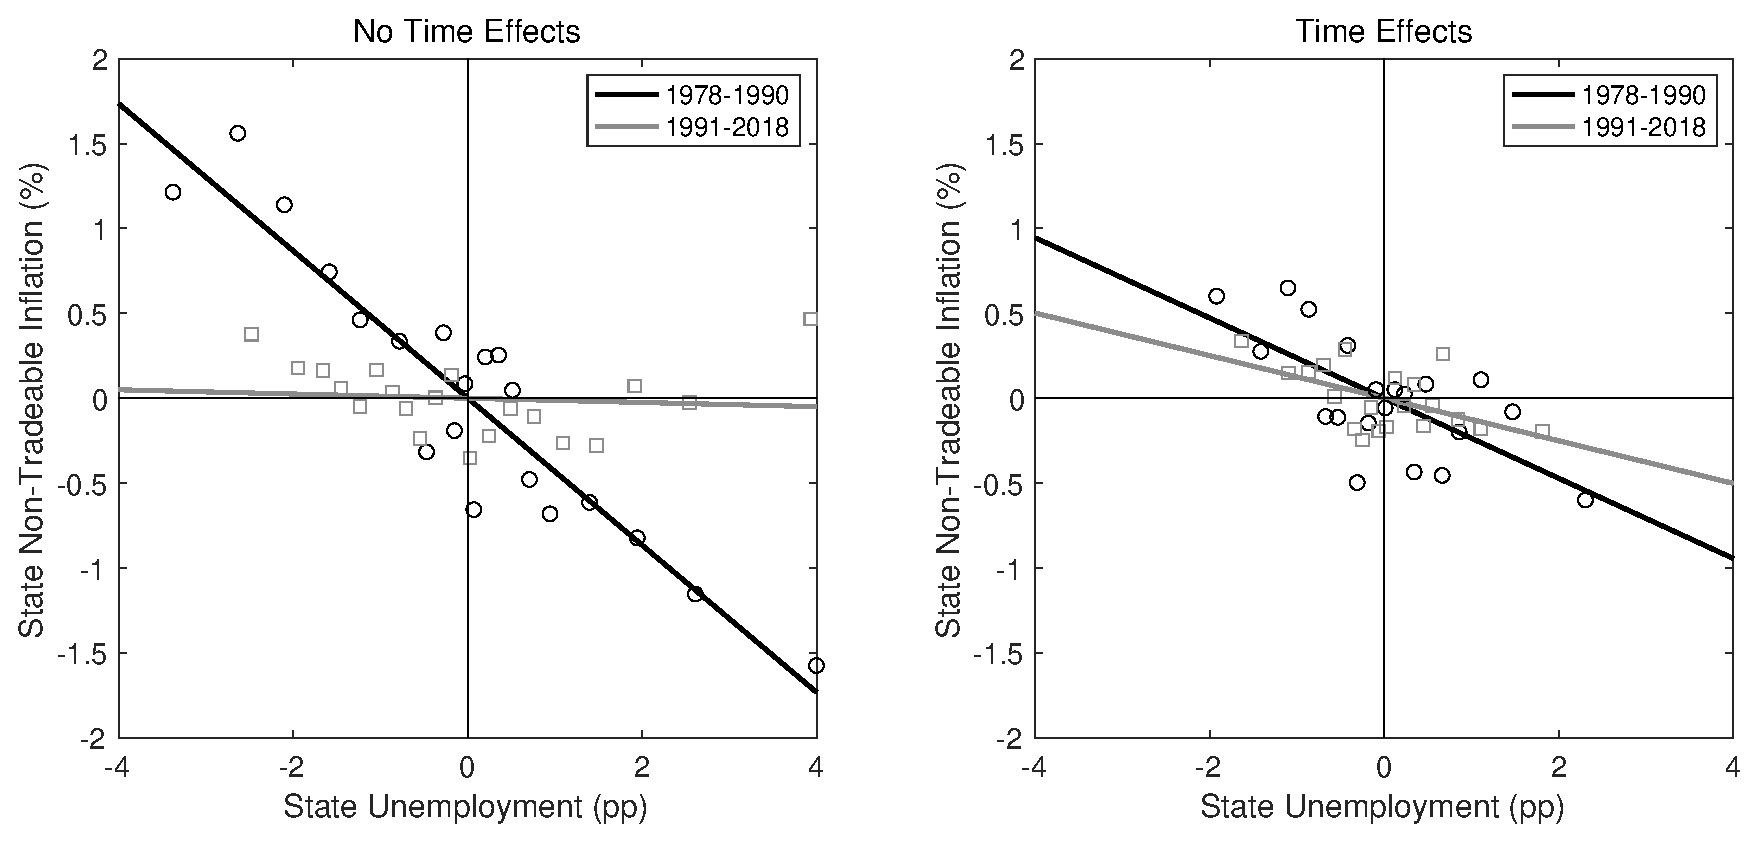
\includegraphics[width=1.0\textwidth]{FiguresTables/Fig_binscatter.eps}
		\caption{Scatterplots---Non-Tradeable Inflation and Unemployment}
	\end{figure}
\end{frame}



\begin{frame}{Main Conclusions}
	\begin{itemize}
		\itemsep1em 
		\item Slope of Phillips curve small
		\begin{itemize}
			\item $\kappa = 0.0062$ implies that even a 5 percentage point increase in unemployment decreases inflation by only 2 percentage points \\ (if inflation expectations remain unchanged)
		\end{itemize}
		\item Apparent ``flattening'' mainly due to anchoring of expectations
		\begin{itemize}
			\item No time fixed effects: Factor >100 flattening
			\item With time fixed effects: Factor 2 flattening \vspace{2mm}
			\item Interpretation: Time fixed effects absorb movements in \\ long-run inflation expectations
		\end{itemize}
	\end{itemize}
\end{frame}


\begin{frame}
	\begin{table}
		\centering 
		\small 
		\caption{HHNS Estimates Compared to Prior Work} \vspace{-5pt}
		\begin{tabular}{p{5.5cm}c} \hline \hline
			& $\kappa$ \\ \hline \\ [-2mm]
			Gali (2008) & 0.085 \\
			Rotemberg and Woodford (1997) & 0.019 \\
			Nakamura and Steinsson (2014) & 0.0077 \\ \\ [-2mm]
			\textbf{Our Estimate} \\
			Full Sample IV Estimate & 0.0062 \\ \\ [-2mm] \hline
		\end{tabular}
		\begin{minipage}[c]{4in}
			\footnotesize \baselineskip=11pt \vspace{5pt}
			Note: HHNS adjust prior estimates by the elasticity of output with respect to employment in the model in these papers. For Nakamura and Steinsson (2014), HHNS use the calibration with GHH preferences. 
		\end{minipage}
	\end{table}
\end{frame}


\begin{frame}{Missing Disinflation?}
	\begin{itemize}
		\itemsep1em 
		\item Can HHNS's cross-section estimate of $\kappa$ explain aggregate time-series fluctuations in inflation?
		\item Many have argued:
		\begin{itemize}
			\item Missing disinflation during Great Recession
			\item Missing reinflation during late 2010s and late 1990s
		\end{itemize}
		\item Are cross-sectional estimates of Phillips curve steeper than \\ time-series estimates?
	\end{itemize}
\end{frame}


\begin{frame}{Aggregate Implication}\label{agg_impl}
	\begin{itemize}
		\itemsep1em 
		\item Plot RHS and LHS of
		\[ \pi_{t} - E_{t}\pi_{t+\infty} =-\kappa \zeta \tilde{u}_{t} + \omega_t\]
		assuming no supply shocks $\omega_t = 0$
		\item Scaling factor: $\zeta = 6.16$ (s.e. 1.80)
		\[\sum_{j=0}^{T} \beta^j \tilde{u}_{t+j} = \zeta \tilde{u}_{t} + \alpha + \epsilon_{t}. \]
		\item Aggregate includes housing 
		\begin{itemize}
			\item Estimate aggregate Phillips curve for shelter
			\item Data from American Community Survey for 2001-2017
			\item $\kappa = 0.0243$ (s.e. 0.0053)
			\item About four time larger than for non-shelter
		\end{itemize}
	\end{itemize}
\end{frame}



\begin{frame}[label=flatflatter]
	\vspace{30pt}
	\begin{figure}[t]
		\centering
		\includegraphics[width = 0.65\textwidth]{FiguresTables/fit_pc_ppt_housing.eps}
		\caption{Aggregate Phillips Curve}
	\end{figure}
\end{frame}

\begin{frame}{Has Phillips Curve ``Broken Down'' Recently?}
	\begin{itemize}
		\itemsep1em 
		\item Post-1990: Predictions fit data reasonably well
		\begin{itemize}
			\item Essentially no missing disinflation or missing reinflation
		\end{itemize}
		\item Pre-1990: Data deviates substantially from predictions
		\begin{itemize}
			\item Actual inflation gap much higher than predicted
			\item Natural Explanation: Adverse supply shocks 
		\end{itemize}
		\item Opposite of conventional wisdom
	\end{itemize}
\end{frame}



\begin{frame}{The Elephant in the Room}
	\begin{itemize}
		\itemsep1em 
		\item Key determinant of inflation: $E_t \pi_{t+\infty}$
		\item But how does the monetary authority change $E_t \pi_{t+\infty}$ 
		\begin{itemize}
			\item Fundamentally hard!!
			\item How does it convince people that what it says is credible?
			\item Answering this is not a strong suit of economists (need more research)
		\end{itemize}
		\item Sometimes beliefs do change rapidly \\ (e.g., Volcker disinflation, ends of hyperinflations)
	\end{itemize}
\end{frame}

\begin{frame}{How Does One Change Long-Run Beliefs?}
	\begin{itemize}
		\itemsep1em 
		\item Volcker tightened policy dramatically
		\begin{itemize}
			\item Caused massive recession
			\item Didn't get fired 
		\end{itemize}
		\item Perhaps this was crucial in changing beliefs about \\ long-run monetary regime
		\item Fundamentally different from view that inflation fell \\ due to steep Phillips curve	
	\end{itemize}
\end{frame}


\end{document}










